\documentclass{article}

% if you need to pass options to natbib, use, e.g.:
%     \PassOptionsToPackage{numbers, compress}{natbib}
% before loading neurips_2020

% ready for submission
% \usepackage{neurips_2020}

% to compile a preprint version, e.g., for submission to arXiv, add add the
% [preprint] option:
%     \usepackage[preprint]{neurips_2020}

% to compile a camera-ready version, add the [final] option, e.g.:
%     \usepackage[final]{neurips_2020}

% to avoid loading the natbib package, add option nonatbib:
     \usepackage[nonatbib]{neurips_2020}

\usepackage[utf8]{inputenc} % allow utf-8 input
\usepackage[T1]{fontenc}    % use 8-bit T1 fonts
\usepackage{hyperref}       % hyperlinks
\usepackage{url}            % simple URL typesetting
\usepackage{booktabs}       % professional-quality tables
\usepackage{amsfonts}       % blackboard math symbols
\usepackage{nicefrac}       % compact symbols for 1/2, etc.
\usepackage{microtype}      % microtypography
\usepackage{graphicx}

\title{CSC 480 Final Project Report}

% The \author macro works with any number of authors. There are two commands
% used to separate the names and addresses of multiple authors: \And and \AND.
%
% Using \And between authors leaves it to LaTeX to determine where to break the
% lines. Using \AND forces a line break at that point. So, if LaTeX puts 3 of 4
% authors names on the first line, and the last on the second line, try using
% \AND instead of \And before the third author name.

\author{%
  Shawn Kim \\
  CSC 480: Principals of Machine Learning\\
  University of Arizona\\
  \texttt{tkim1@arizona.edu} \\
  % examples of more authors
  % \And
  % Coauthor \\
  % Affiliation \\
  % Address \\
  % \texttt{email} \\
  % \AND
  % Coauthor \\
  % Affiliation \\
  % Address \\
  % \texttt{email} \\
  % \And
  % Coauthor \\
  % Affiliation \\
  % Address \\
  % \texttt{email} \\
  % \And
  % Coauthor \\
  % Affiliation \\
  % Address \\
  % \texttt{email} \\
}

\begin{document}

\maketitle

% \begin{abstract}
%   The abstract paragraph should be indented \nicefrac{1}{2}~inch (3~picas) on
%   both the left- and right-hand margins. Use 10~point type, with a vertical
%   spacing (leading) of 11~points.  The word \textbf{Abstract} must be centered,
%   bold, and in point size 12. Two line spaces precede the abstract. The abstract
%   must be limited to one paragraph.

%   This final report aims to demonstrate some of the fundamental techniques of
%   computer vision through exploring the problem of correctly classifying images
%   of handwritten digits from one to through ten. A combination of relevant
%   preprocessing techniques and machine learning algorithms in computer vision
%   will be utilized to achieve this goal. The methodology that produced the best
%   performing score(s) will then be dissected to get an intuition of the impact
%   of each step in the training process. Finally, future directions and
%   additional experiments will be discussed.

%   The Kannada MNIST competition tasks you with the computer vision problem of
%   recognizing images of hand-written Kannada digits from one through
%   ten. Kannada is a language spoken by the people of Karnataka in southwestern
%   India. This competition is a variant of the classic MNIST digit recognizer
%   case study in computer vision. The performance metric being used is the
%   percentage of hand-written Kannada digit images correctly classified.
% \end{abstract}
\section{Introduction}

The Kannada MNIST competition presents a computer vision challenge involving the
recognition of handwritten Kannada digits from zero to nine. Kannada is a
language spoken by the inhabitants of Karnataka, a state in southwestern
India. This competition is a variation of the original MNIST digit classifier
case study that worked with arabic numerals from zero to nine. The evaluation
metric for Kannada digit classification is the percentage of handwritten Kannada
digits accurately classified.

The motivation for this project is to explore fundamental machine learning
concepts in computer vision. This problem presents not only an opportunity to
apply and practice material that we have directly covered in class but also
serves as a good introduction to computer vision as a whole. The programming
environment of choice for this project will be MATLAB, and all work is done in
MATLAB.

\section{Background}

The task is to train a classifier that can correctly label all hand-written
Kannada digits. This will be done by using a two step process of first
preprocessing the images and then feeding the pre-processed images into a
machine learning algorithm.

The dataset itself consists of around 75,000 grayscale images of which 10,000
are reserved for the validation set and of which 5,000 are reserved for the
testing set. Each image is 28 by 28 pixels for a total of 784 pixels per
image. Since the images are grayscale, each pixel has one channel that
represents the intensity value of the pixel rather than three color channels for
RGB. The intensity value itself ranges from 0 to 255.

In Figure 1, the first set of zero to nine hand-written Kannada digits in the
training set are visualized to get an intuition of the dataset.

\begin{figure}[h]
  \centering
  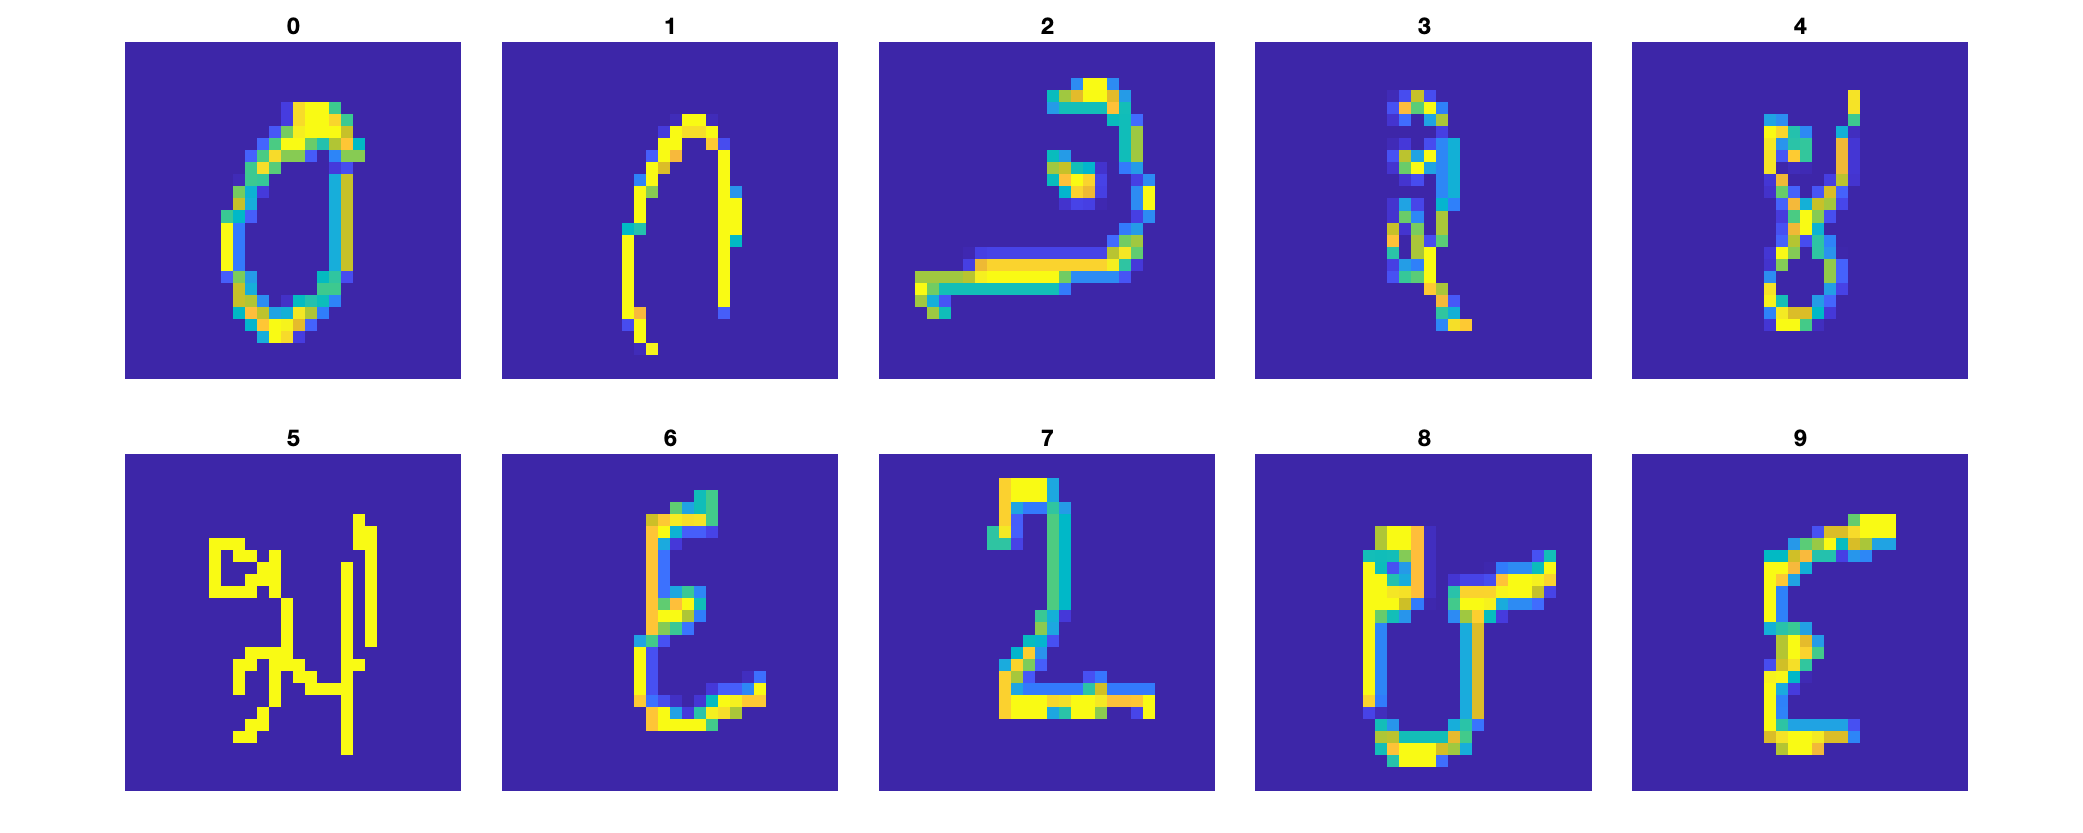
\includegraphics[width=0.65\linewidth]{digits.png}
  \caption{In MATLAB, the first set of zero to nine hand-written Kannada digits
    in the training set is visualized using the MATLAB \texttt{imagesc()}
    function. This function automatically scales up small images to a viewable
    size (like our 28 by 28 pixel images) and maps grayscale values to colors
    based on a colormap for easier distinguishability.}
\end{figure}

\section{Approaches}

The machine learning models used on the dataset are K-nearest neighbors (KNN)
and a convolutional neural network (CNN). The preprocessing techniques used are
normalization, principal component analysis (PCA), and Canny edge detection for
KNN and normalization and data augmentation for CNN.

\subsection{Preprocessing}

The preprocessing techniques as they apply to each respective machine learning
model is discussed.

\subsubsection{Normalization}

Normalization was performed on the dataset. This negates effects like lighting
inconsistencies in the images which can be considered as a kind of noise in the
dataset. KNN relies on distance metrics (Euclidean distance) to determine the
“nearness” of data points. If features have different scales, those with larger
ranges can disproportionately affect the distance calculation, leading to biased
results. Normalization is also standard for CNNs in the form of input
normalization, batch normalization, and layer normalization in order to
stabilize training, prevent vanishing/exploding gradients, and improve
generalization of features.

A normalized dataset (so that all grayscale values were in the range \( [0, 1]\)
for each image) was achieved in MATLAB via the \texttt{normalize()} function.

\subsubsection{Princple Component Analysis}

PCA was performed on the normalized dataset to be used for KNN. PCA is a useful
preprocessing technique for KNN because it reduces the dimensionality of the
dataset. This can help speed up computation and potentially improve the
performance of KNN by removing noisy or less informative features. PCA
however is not a good preprocessing technique for CNN as a CNN inherently learns
feature representations on its own which makes PCA redundant and unncecesary.

PCA on the dataset was performed in MATLAB via the \texttt{pca()} function. The
number of principal components was decided by whatever amount explained at least
95\% of the variance. For the training dataset, this resulted in 237 principal
components which is a considerable reduction in dimensionality remembering that
the original flattened image vector was 784 pixels for each image.

In Figure 2, a pareto chart of the first ten principal components of the
training dataset is shown.

\begin{figure}
  \centering
  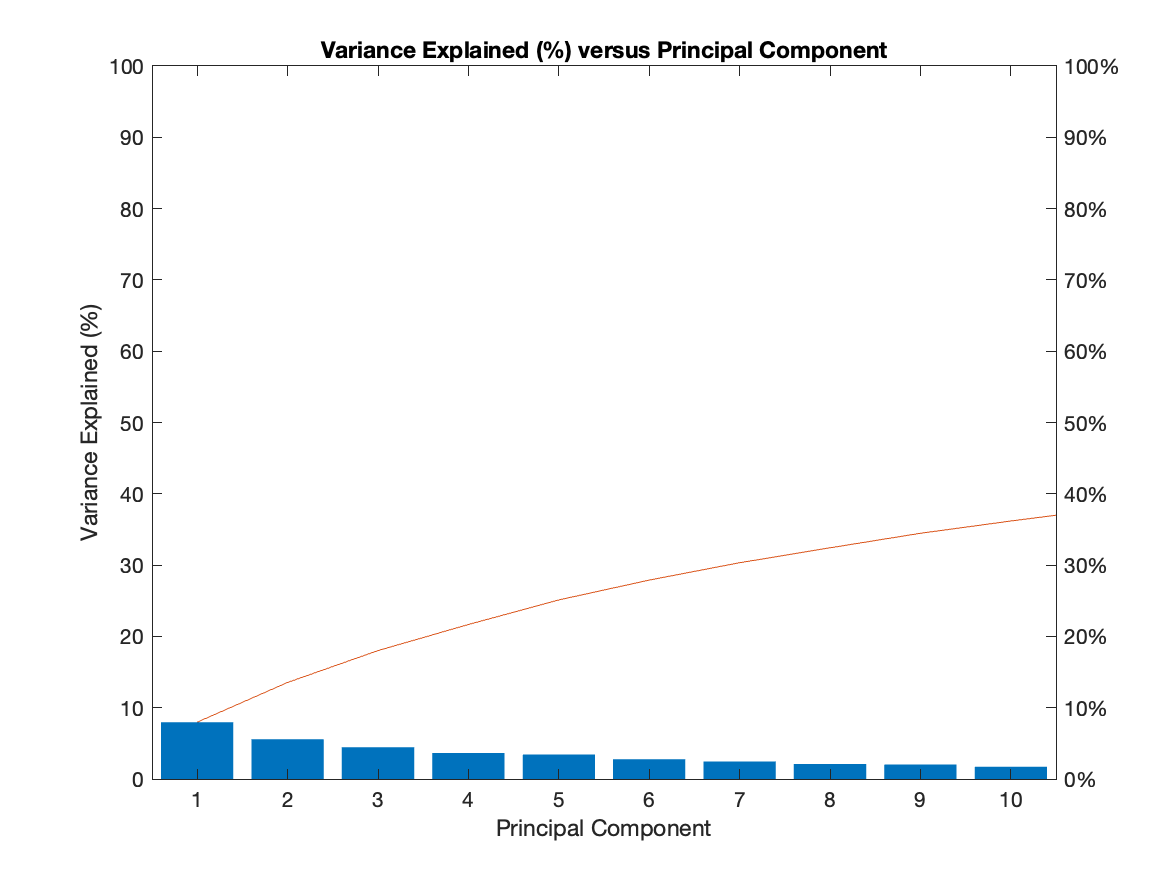
\includegraphics[width=0.65\linewidth]{pca.png}
  \caption{In MATLAB, the variance explained versus principal component pareto
    chart is generated with the \texttt{pareto()} function. The first ten
    principal components are shown to have a combined explained variance of
    close to 40\%.}
\end{figure}

\subsubsection{Canny Edge Detection}

Canny edge detection was also performed on the normalized dataset to be used for
KNN. Canny edge detection is useful for KNN because it reduces the input
complexity by focusing only on edges, and edges capture the digit’s shape and
outline, which are critical for classification. Like PCA, Canny edge detection
was not used for CNN as a CNN inherently learns edge-like features on its own.

Canny edge detection was performed in MATLAB via the \texttt{edge()}
function. Canny edge detection results in a mappinng of pixel grayscale
intensity values to 1 if the pixel lies an edge or 0 if otherwise.

In Figure 3, the same set of zero to nine hand-written Kannada digits from
Figure 1 is now visualized after Canny edge detection.

\begin{figure}
  \centering
  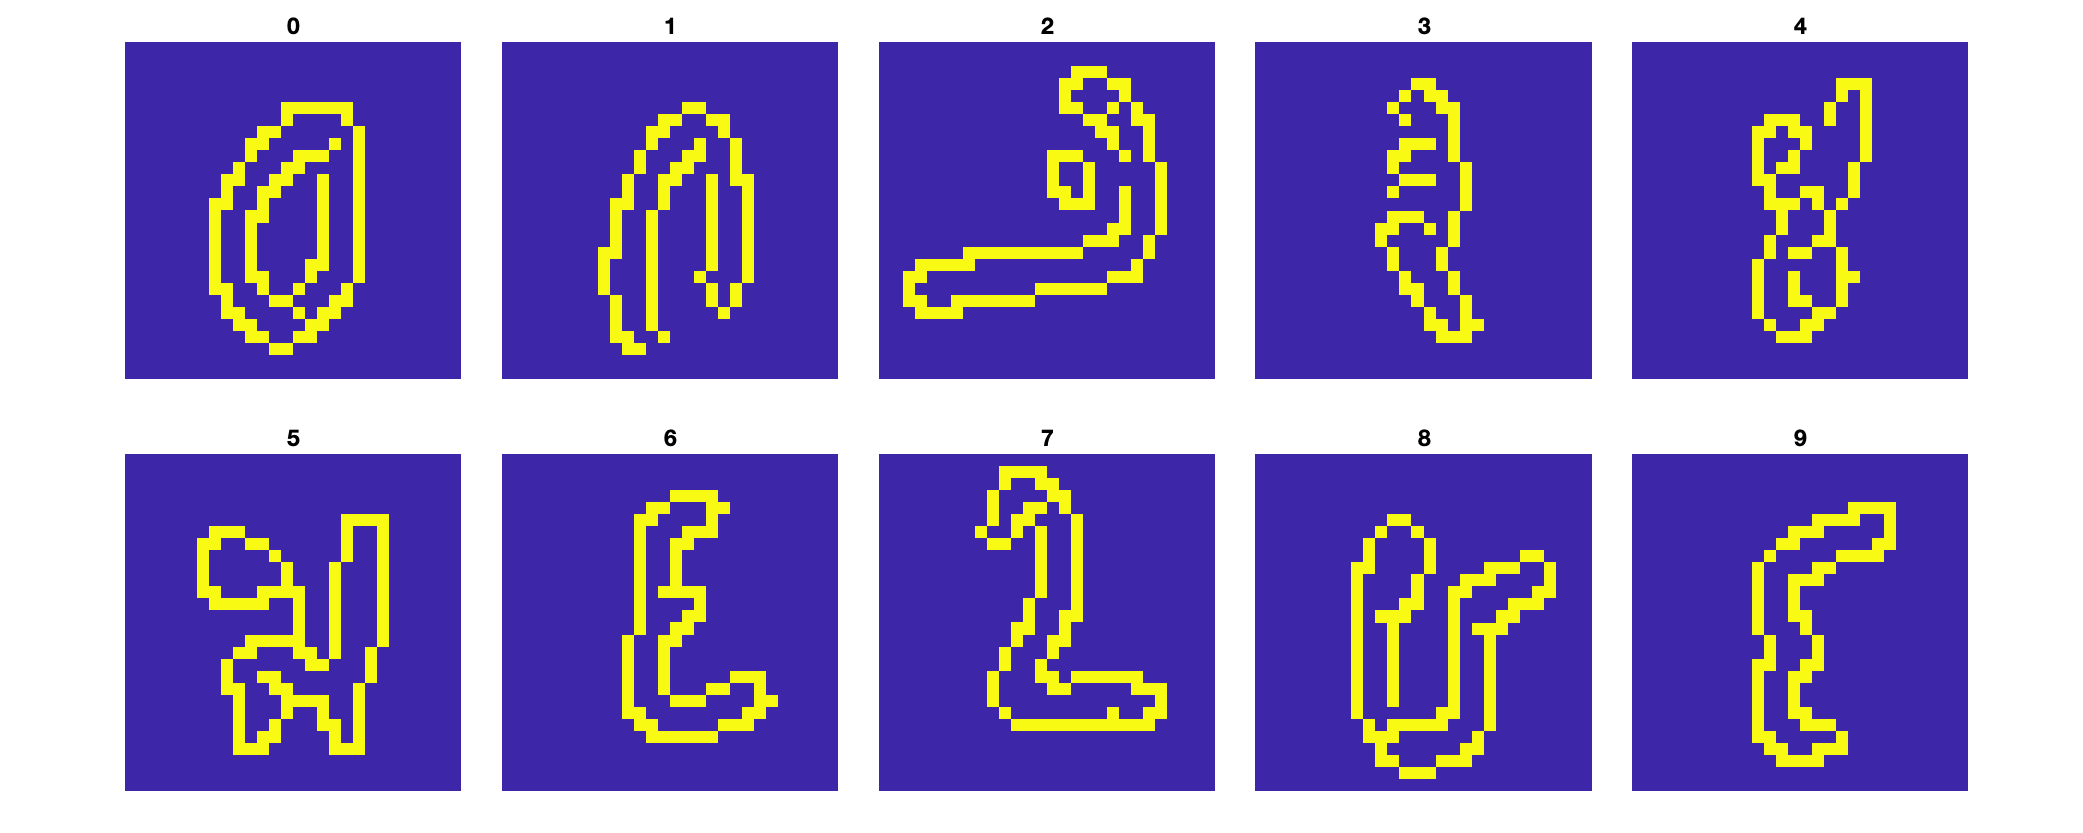
\includegraphics[width=0.65\linewidth]{edge.png}
  \caption{In MATLAB, the edge feature of our previous Figure 1 digit set is
    generated with the \texttt{edge()} function. The edges of the digits are
    shown in yellow which is the max intensity value in the \texttt{imagesc()}
    colormap.}
\end{figure}

\subsubsection{Combining Principal Component Analysis and Canny Edge Detection}

PCA and Canny edge detection can be combined since one is a dimensionality
reduction technique while the other is a (surprise) edge detection technique.

Canny edge detection was fed into PCA to achieve a dimensionality reduction of
the edge features. This resulted in 337 principal components to explain 95\% of
the variance for the training set which is notably higher than the 237 principal
components for just PCA as previously explained.

% I would have expected less principal components after edge detection since we
% are just working with edges, and I am unsure why the opposite is true.

In reverse, PCA fed into Canny edge detection would be an edge detection on the
principal components of the image vector, but in practice, the dataset projected
onto its principal components do not represent an image. Edge detection would
not yield anything meaningful in this case.

\subsubsection{Data Augmentation}

Data augmentation was performed on the dataset to be used with our CNN. Data
augmentation is a crucial technique for improving the performance of CNNs by
artificially expanding the training dataset and making the model more robust to
variations in data.

For the Kannada MNIST digit dataset, the augmentation techniques incorporated
were transformations like random rotation in the angle range \([-45, 45]\),
random scaling indepedently in the X and Y directions in the scaling range
\([0.75,1.25]\), and random translations independently in the X and Y directions
in the range pixel range \([-2,2]\). The newly augmented training dataset
consisted of 120,000 images, 60,000 from the original and another 60,000 that
were augmented from the original.

In Figure 4, data augmentation of our previous Figure 1 digit set is shown.

\begin{figure}
  \centering
  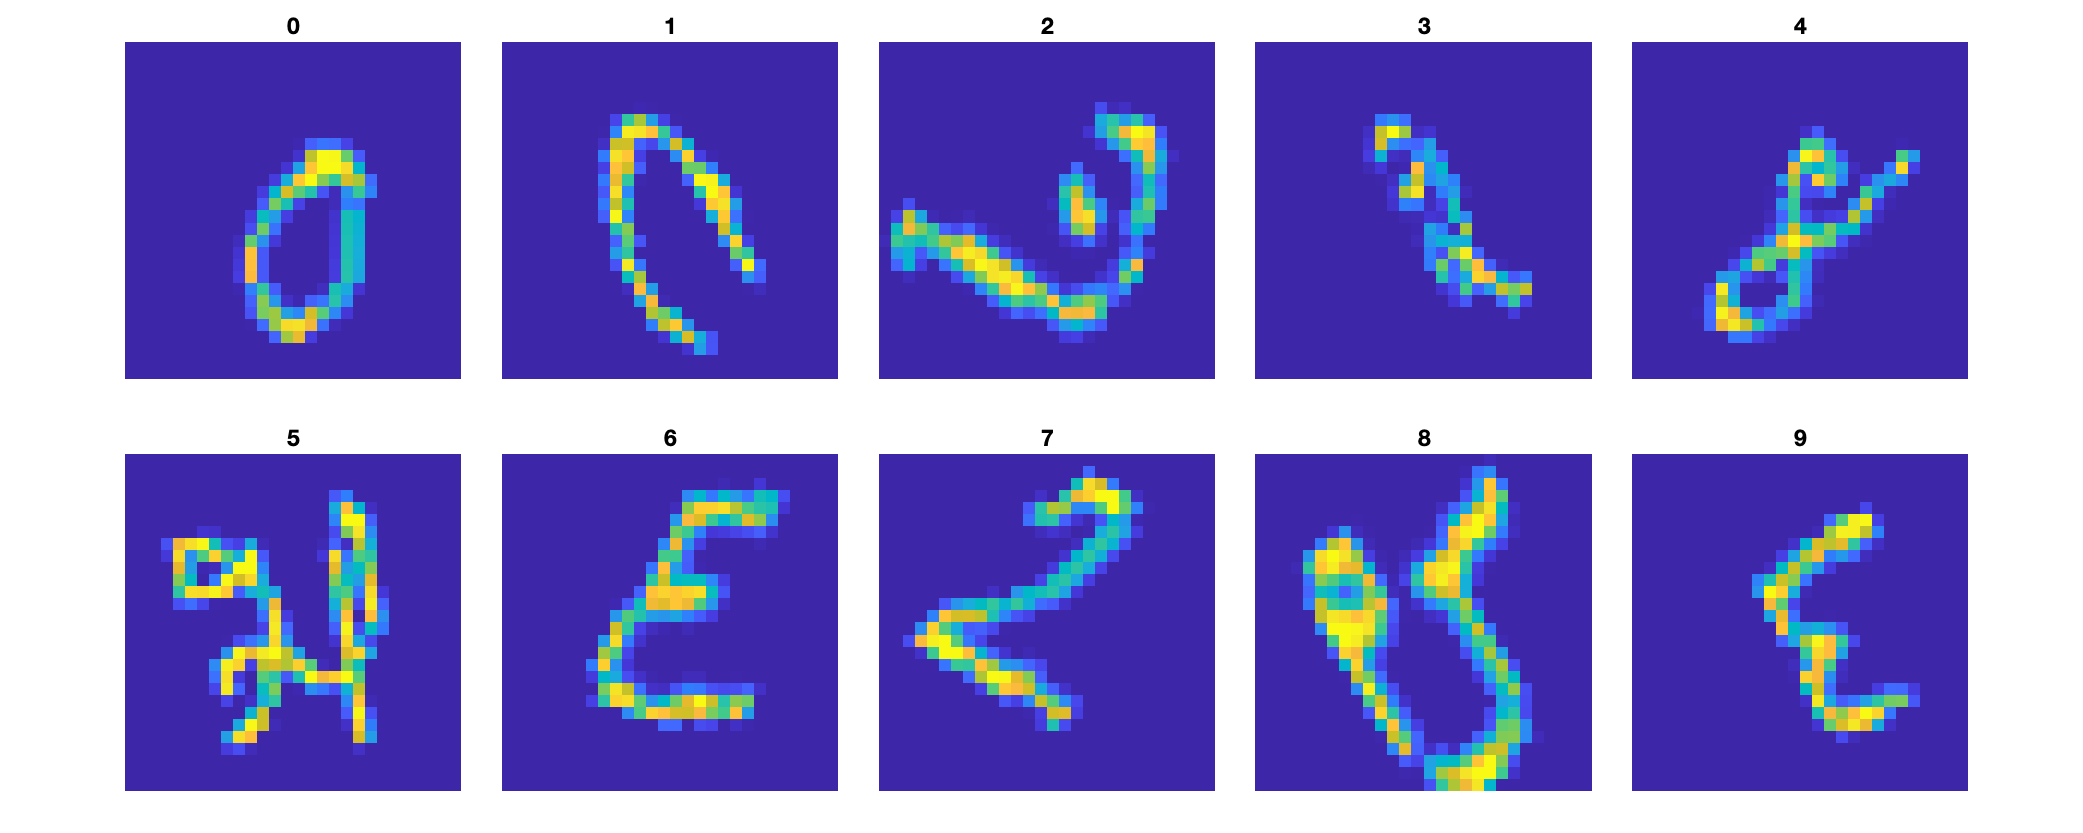
\includegraphics[width=0.65\linewidth]{aug1.png}
  \caption{In MATLAB, data augmentation of our previous Figure 1 digit set is
    produced using functions \texttt{dataImageAugmenter()} and
    \texttt{augment()}. You can see the transformed images realistically mimic
    real variations in human handwriting to give our CNN a more robust dataset.}
\end{figure}

\subsection{Model Results}

An overview of how each of the models (KNN and CNN) was used and their results
is discussed.

\subsubsection{KNN}
For KNN, \(k=3,5,7\) were trained with the normalized, PCA, Canny edge, and
Canny edge into PCA training datasets using \texttt{fitcknn()}. The results on
the test dataset are shown in Table 1.

\begin{table}[h]
  \caption{KNN Test Accuracy Results (\%)}
  \centering
  \begin{tabular}{llll}
    \toprule
    % \multicolumn{4}{c}{Part}                   \\
    % \cmidrule(r){2-4}
    Dataset & k=3 & k=5 & k=7 \\
    \midrule
    Non-normalized & 71.90 & 71.46 & 71.09\\
    Normalized & 71.90 & 71.46 & 71.09 \\
    PCA & \ \ 5.16 & \ \ 5.19 & \ \ 5.12 \\
    Canny edge & 62.08 & 61.82 & 61.89\\
    Canny edge/PCA & 13.05 & 13.49 & 13.59\\
    \bottomrule
  \end{tabular}
\end{table}

It appears that the normalized/non-normalized training dataset achieved the
highest overall accuracy on the testing dataset. The fact that the accuracy does
not change between normalized and non-normalized training data makes sense
because normalizing the images just scaled every pixel value down and did not
change the Euclidean distance metric of KNN.

It also appears that PCA had the worse performing score. This indicates that PCA
discarded important features of the dataset even though it was supposed to keep
the most important ones. PCA may not have been the best preprocessing technique
for our dataset since images were already relatively small (28 by 28 pixels), so
it could have been that all 784 pixels of information per image was necessary
for KNN to do somewhat well.

Canny edge had the second highest peforming score but was still lower than
normalized/non-normalized score. This is consistent with what is observed for
PCA because, again, Canny edge detection filters the image to only retain the
edges of the digits which means that other features of the digits are lost. It
appears that our digit images are too small in size for advanced preprocessing
techniques to be effective.

Canny edge into PCA has an expected much lower score than just Canny edge
because PCA further discards information from the edge features that Canny edge
detection filtered from the original images.

Overall, PCA and Canny edge did no favors for KNN. KNN performed the best with
all the pixel information which intuitively makes sense because KNN is trying to
make a classification based on how close the pixels are to the label samples it
has already seen.

\subsubsection{CNN}

For CNN, the MATLAB deep learning toolbox was used to program a CNN consisting
of 5 layers; an input layer, 3 convolutional layers, and a fully connected
layer.

The input layer was defined for 28 by 28 grayscale images. The first
convolutional layer used 3 by 3 kernels with 8 filters and padding to preserve
the spatial size of the image. Batch normalization was applied after each
convolution layer to normalize activations, and Rectified Linear Unit (ReLU) was
used as the activiation function after each convolution. Furthermore, max
pooling with a stride of 2 was also applied after each convolution to reduce
spatial dimensions by a factor of 2. The fully connected layer had 10 units
corresponding to the 10 labels of 1 through 9. Softmax was used to output the
probabilities for each of the classes which was then fed into a classification
layer for final decision. For CNN training, an Adam optimizer was set with a
learning rate of 0.001, and the number of training epochs was set to 5.

In Table 2, the test results of the CNN trained on the non-augmented and
augmented datasets are shown. Both the non-augmented and augmented datasets are
normalized.

\begin{table}[h]
  \caption{CNN Test Accuracy Results (\%)}
  \centering
  \begin{tabular}{lll}
    \toprule
    Dataset & Accuracy & Training Time \\
    \midrule
    Non-augmented & 75.57 & 1m49s\\
    Augmented & 87.28 & 3m43s\\
    \bottomrule
  \end{tabular}
\end{table}

It appears that CNN was slightly more effective than KNN when using just the
normalized, non-augmented dataset. With the augmented dataset however, test
accuracy increased by almost 12\% which shows that augmentation of the digit
dataset was indeed effective for CNN.

\section{Ablation Study}

Since CNN was the best peforming model, an ablation study was done to experiment
with the convolutional layers of the CNN versus the dataset. The ablation study
was performed by first adding a layer and then gradually removing layers from
the model and training on the augmented and non-augmented datasets to see what
happened. This is reported in Table 3.

\begin{table}[h]
  \caption{CNN Test Accuracy Results (\%)}
  \centering
  \begin{tabular}{lll}
    \toprule
    Convolutional Layer(s) & Augmented & Non-augmented \\
    \midrule
    Four Layers & 85.31 & 76.77\\
    Three Layers & 87.28 & 75.57\\
    Two Layers & 84.22 & 72.90\\
    One Layer & 77.54 & 70.01\\
    \bottomrule
  \end{tabular}
\end{table}

Since more convolutional layers results in more hierarchical features of the
image being learned, in theory, the testing accuracy should go down as the
layers are removed. This seems to generally be the case for both the augmented
and non-augmented datasets except for four convolutional layers with the
augmented dataset. This goes to show that fine-tuning a CNN is not just simply
adding more layers to the model, although it certainly does help up to three
layers based on my findings.

\section{Future Directions}

In the future, I would like to experiment on improving the performance of KNN
with other preprocessing techniques such Scale Invariant Feature Transform
(SIFT) vectors which seem promising for Euclidean distance KNN. I would also try
and experiment with the KNN training times, although I think this avenue is
limited since KNN needs to work with increasingly highy dimensional vectors to
increase accuracy, or so it seems based on my results.

For CNN, I would like to look into expanding the size and improving the
robustness of augmentations on the dataset as my experiments have shown that
they have a great, positive impact on the accuracy of the CNN. I would also like
explore other avenues of image preprocessing that can further increase the
quality of the dataset like with data augmentation.

In general, I would also try to do the machine learning on my Windows PC next
time since it actually has a GPU for machine learning rather than doing it on my
MacBook which just uses the CPU.

\end{document}
